\begin{pastexam}[label={px:gk3-096-ds-01}]{高考三級資訊處理 96 年 第一題}
（申論；25 分）

圖（graph）的表示法（Graph Representation）
\begin{itemize}[leftmargin=2.2em]
\item[㈠] 以下面的無向圖（undirected graph）為例，說明圖的鄰接串列（adjacency list）表示法。（10 分）

\begin{center}
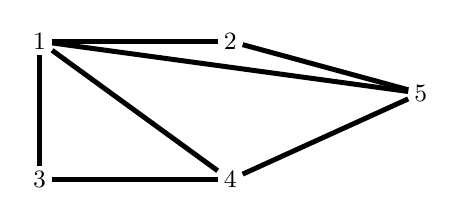
\begin{tikzpicture}[x=1.1cm,y=1.1cm,v/.style={inner sep=2pt,font=\small}]
\node[v] (1) at (0,1.6) {1};
\node[v] (2) at (2.2,1.6) {2};
\node[v] (5) at (4.4,1.0) {5};
\node[v] (3) at (0,0) {3};
\node[v] (4) at (2.2,0) {4};
\draw[line width=1.8pt] (1)--(2);
\draw[line width=1.8pt] (1)--(5);
\draw[line width=1.8pt] (1)--(3);
\draw[line width=1.8pt] (1)--(4);
\draw[line width=1.8pt] (3)--(4);
\draw[line width=1.8pt] (2)--(5);
\draw[line width=1.8pt] (4)--(5);
\end{tikzpicture}
\end{center}
\item[㈡] 以下面的有向圖（directed graph）為例，說明圖的鄰接矩陣（adjacency matrix）表示法。（5 分）

\begin{center}
\begin{tikzpicture}[x=1.1cm,y=1.1cm,v/.style={inner sep=2pt,font=\small},>={Triangle[length=2.2mm]}]
\node[v] (1) at (0,1.6) {1};
\node[v] (2) at (2.2,1.6) {2};
\node[v] (5) at (4.4,1.0) {5};
\node[v] (3) at (0,0) {3};
\node[v] (4) at (2.2,0) {4};
\draw[->] (2)--(1);
\draw[->] (1)--(5);
\draw[->] (5)--(2);
\draw[->] (1)--(4);
\draw[->] (3)--(1);
\draw[->] (3)--(4);
\draw[->] (5)--(4);
\end{tikzpicture}
\end{center}
\item[㈢] 給一 $n$ 個節點（vertex）的有向圖 $G$ 的鄰接矩陣，請問計算圖 $G$ 的一個節點的出分支度（out degree）的時間複雜度為何？（5 分）
\item[㈣] 給一 $n$ 個節點（vertex）的有向圖 $G$ 的鄰接矩陣，請簡述判斷圖 $G$ 是否連通（connected）的演算法。（5 分）
\end{itemize}
\end{pastexam}

\begin{pastsoln}
兩種表示法見資結書第~21.2~節。 圖上的點本書照原題叫「節點」。

\textbf{㈠ 鄰接串列}。 每個節點 $v$ 有一條串列，串著所有和 $v$ 相鄰的節點；$n$ 條串列的開頭放在
一個長度 $n$ 的陣列 $\mathit{adj}[1..n]$ 裡。 無向邊 $\{u, v\}$ 在 $u$ 的串列和 $v$ 的串列各出
現一次。 這張圖有 $7$ 條邊：$\{1,2\}$、$\{1,3\}$、$\{1,4\}$、$\{1,5\}$、$\{2,5\}$、$\{3,4\}$、$\{4,5\}$。
串列裡的節點依編號由小到大排（題目沒有規定順序，任何順序都表示同一張圖）：
\begin{center}
\begin{tikzpicture}[x=1.05cm,y=0.62cm,h/.style={draw,minimum width=7mm,minimum height=4.6mm,inner sep=0pt,font=\small},
  c/.style={draw,minimum width=6mm,minimum height=4.6mm,inner sep=0pt,font=\small},
  p/.style={draw,minimum width=3.5mm,minimum height=4.6mm,inner sep=0pt},>={Stealth[length=1.8mm]}]
\foreach \v/\lst [count=\r] in {1/{2,3,4,5}, 2/{1,5}, 3/{1,4}, 4/{1,3,5}, 5/{1,2,4}} {
  \node[h] (h\r) at (0,-\r) {\v};
  \foreach \u [count=\k] in \lst {
    \node[c] (c\r-\k) at (1.3*\k,-\r) {\u};
    \node[p,anchor=west] (p\r-\k) at (c\r-\k.east) {};
  }
}
\foreach \r/\m in {1/4, 2/2, 3/2, 4/3, 5/3} {
  \draw[->] (h\r.east) -- (c\r-1.west);
  \foreach \k [evaluate=\k as \kk using int(\k+1)] in {1,...,\m} {
    \ifnum\k<\m \draw[->] (p\r-\k.center) -- (c\r-\kk.west); \fi
  }
  \node[font=\scriptsize] at (p\r-\m.center) {$\wedge$};
}
\node[font=\small] at (0,-0.25) {$\mathit{adj}$};
\end{tikzpicture}
\end{center}
每個串列節點有兩欄：鄰居的編號和指向下一個節點的指標，最後一個的指標是 $\NIL$（圖裡畫成
$\wedge$）。 串列節點總共 $4 + 2 + 2 + 3 + 3 = 14 = 2 \times 7$ 個，也就是度數總和等於邊數的
兩倍（資結書定理~21.1，握手定理）。 一般來說鄰接串列用 $\Theta(n + m)$ 的空間（$m$ 是邊數），
列出 $v$ 的所有鄰居要 $\Theta(\deg(v))$ 時間，適合邊少的稀疏圖。

\textbf{㈡ 鄰接矩陣}。 用 $n \times n$ 的陣列 $A$，有向邊 $u \to v$ 存在時 $A[u][v] = 1$，否則
是 $0$。 列是邊的起點、行是終點。 這張圖的 $7$ 條有向邊是 $1 \to 4$、$1 \to 5$、$2 \to 1$、
$3 \to 1$、$3 \to 4$、$5 \to 2$、$5 \to 4$：
\[
A = \bordermatrix{
  & 1 & 2 & 3 & 4 & 5 \cr
1 & 0 & 0 & 0 & 1 & 1 \cr
2 & 1 & 0 & 0 & 0 & 0 \cr
3 & 1 & 0 & 0 & 1 & 0 \cr
4 & 0 & 0 & 0 & 0 & 0 \cr
5 & 0 & 1 & 0 & 1 & 0 \cr}
\]
有向圖的矩陣一般不對稱（例如 $A[2][1] = 1$ 但 $A[1][2] = 0$）；無向圖的矩陣一定對稱。 矩陣
有 $7$ 個 $1$，正好是邊數。 鄰接矩陣用 $\Theta(n^2)$ 空間，判斷 $u \to v$ 是否存在只要 $O(1)$。

\textbf{㈢ 出分支度}。 節點 $u$ 的出分支度是以 $u$ 為起點的邊數，就是第 $u$ 列 $1$ 的個數：
\[
\deg^{+}(u) = \sum_{v=1}^{n} A[u][v].
\]
一列有 $n$ 格，每格都要看（任何一格沒看，那一格可能是 $1$），所以時間是 $\Theta(n)$。 例如上圖
$\deg^{+}(1) = 0 + 0 + 0 + 1 + 1 = 2$。 （入分支度則是第 $u$ 行的和，也是 $\Theta(n)$。）

\textbf{㈣ 連通}。 有向圖的「連通」有兩種意思，兩種都寫：
\begin{itemize}
\item \textbf{弱連通}：把邊的方向拿掉以後連通。 做法是從節點 $1$ 做 BFS（或 DFS），把 $A[u][v] = 1$
\textbf{或} $A[v][u] = 1$ 都當成 $u$、$v$ 相鄰。 搜尋結束時所有節點都被走到，就是（弱）連通。
\item \textbf{強連通}：任兩個節點 $u$、$v$ 之間 $u$ 能走到 $v$、$v$ 也能走到 $u$。 做法是做兩次搜尋：
第一次從節點 $1$ 沿著邊的方向（看第 $u$ 列的 $A[u][v]$）走，檢查是否走到全部節點；第二次從節點
$1$ 逆著邊的方向（看第 $u$ 行的 $A[v][u]$，等於在轉置圖上走）走，再檢查一次。 兩次都走到全部
節點，才是強連通。 理由：第一次表示 $1$ 能到每個點，第二次表示每個點能到 $1$，於是任兩點
$u \leadsto 1 \leadsto v$ 互相可達。
\end{itemize}
用鄰接矩陣時，BFS 每取出一個節點就要掃它的整列（或整行）$n$ 格，$n$ 個節點共 $\Theta(n^2)$，
所以兩種判斷都是 $O(n^2)$ 時間。 以 ㈡ 的圖為例：它是弱連通的；但節點 $4$ 的出分支度是 $0$，
從 $4$ 走不到別的點，所以不是強連通。
\begin{pseudo}[unbreakable]{從節點 $s$ 做 BFS，$A$ 是鄰接矩陣（弱連通：相鄰改成 $A[u][v] = 1$ 或 $A[v][u] = 1$）}
\Function{Reach-All}{$A, n, s$}
    \State $\mathit{visited}[1..n] \gets \FALSE$；$\mathit{visited}[s] \gets \TRUE$；$\mathit{cnt} \gets 1$
    \State $Q \gets$ 只有 $s$ 的佇列
    \While{$Q$ 不空}
        \State $u \gets$ \Call{Dequeue}{$Q$}
        \For{$v \gets 1$ \To $n$}
            \If{$A[u][v] = 1$ \AND $\mathit{visited}[v] = \FALSE$}
                \State $\mathit{visited}[v] \gets \TRUE$；$\mathit{cnt} \gets \mathit{cnt} + 1$
                \State \Call{Enqueue}{$Q, v$}
            \EndIf
        \EndFor
    \EndWhile
    \State \Return $\mathit{cnt} = n$
\EndFunction
\end{pseudo}
\end{pastsoln}
